\section{系统架构资源消耗测试}
在系统架构测试中,资源消耗是一个重要的考量因素,特别是在服务端硬件配置需求和服务器架构设计方面。以下是对服务端硬件配置需求和服务器架构的详细描述,以及它们对资源消耗的影响:

\subsection{服务端硬件配置需求}
为了确保医疗预约管理系统的高效运行,服务端硬件配置需求必须满足特定的性能标准。这些需求包括但不限于:

\begin{itemize}
	\item \textbf{处理器(CPU)}:需要足够强大的处理器来处理大量的并发请求和复杂的业务逻辑。
	\item \textbf{内存(RAM)}:充足的内存资源可以保证系统在高负载情况下的流畅运行。
	\item \textbf{存储(HDD/SSD)}:快速的存储设备有助于提高数据读写速度,减少等待时间。
	\item \textbf{网络带宽}:高速的网络连接确保了数据传输的效率,特别是在云服务和远程访问时。
	\item \textbf{冗余和备份}:硬件冗余和备份机制可以提高系统的可靠性和容错能力。
\end{itemize}

合适的硬件配置可以显著降低系统资源的消耗,提高整体性能,从而为用户提供更加流畅的服务体验。

\subsection{服务器架构}
本部分详细介绍医疗预约管理系统服务器端的架构设计,该设计采用了分层架构,具体分为四个层次:Controller层、Service层、Mapper层和Model层。

\begin{figure}[htbp]
	\centering
	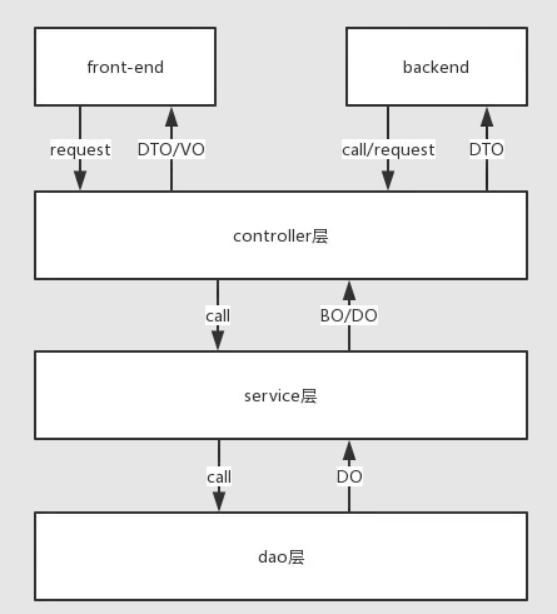
\includegraphics[width=0.5\textwidth]{figures/31.png}
	\caption{代码结构}
\end{figure}

\subsubsection{Controller层}
Controller层负责处理HTTP请求,包括请求的接收、数据的提取与验证、业务逻辑的调用以及响应的构造和异常的处理。此层的设计遵循用户控制原则、减轻记忆负担原则和界面一致性原则,以提升用户体验。

\subsubsection{Service层}
Service层是系统的核心业务逻辑层,细分为事件类、关系类和提醒类三个模块,负责处理用户请求和执行业务逻辑。

\subsubsection{Mapper层(Dao层)}
Mapper层作为数据访问层,提供数据访问接口,使得Service层能够安全、准确地读写数据库中的数据。

\subsubsection{Model层}
Model层包含与数据库表字段相对应的实体类,这些实体类封装了数据,并提供了标准的set/get方法。

合理的服务器架构设计有助于优化资源消耗,提高系统的运行效率和稳定性。通过Service层、Mapper层和Model层的协同工作,医疗预约管理系统能够为病人提供一站式医疗服务,同时确保数据的安全性和稳定性。

在技术实现方面,项目采用了面向对象的设计原则,前端框架的构建是开发团队的主要责任。我们选择了Vue.js作为前端框架,并使用JavaScript作为编程语言,以实现高效、响应式的用户界面。

总体而言,这些功能的实现旨在为病人提供一个无缝、高效的医疗服务体验,同时确保系统的可维护性和可扩展性,满足未来医疗服务领域的变化和需求。